\documentclass[handout]{beamer}

\mode<presentation>
{
  \usetheme{umbc1}
  \setbeamercovered{transparent}
}

\usepackage[english]{babel}
\usepackage[latin1]{inputenc}
\usepackage[T1]{fontenc}

\usepackage[]{datatool, filecontents}
\DTLsetseparator{=}
\DTLloaddb[noheader, keys={key,value}]{values}{./values.dat}
\newcommand{\var}[1]{\DTLfetch{values}{key}{#1}{value}}

\usepackage{tabularray}

\title[RMP v\var{version}]
{Robot Motion Planning}

\subtitle
{Classic Path Planning Algorithms}

\author[Narayanan]
{A.~Narayanan\inst{1}}

\institute[Technical University of Munich]
{
  \inst{1}
  Department of Informatics\\
}

\subject{Slides}
\date{}

\AtBeginSubsection[]
{
  \begin{frame}<beamer>{Outline}
    \tableofcontents[currentsection,currentsubsection]
  \end{frame}
}

\begin{document}
\begin{frame}
    \titlepage
  \end{frame}
  
  \begin{frame}{Outline}
    \tableofcontents
  \end{frame}

  \section{Overview of Classic Path Planning Approaches}

  \begin{frame}
    \begin{itemize}
        \item \textbf{Roadmap} \pause

        Represent the connectivity of the free space by 1-D Curves \pause

        \item \textbf{Cell Decomposition} \pause

        Decompose the free space into simple cells and represent the connectivity of the free space by adjacency graph of these cells \pause

        \item \textbf{Potential Field} \pause

        Define a potential function over the free space that has a global minimum at the goal and follow the steepest descent of the potential function
    \end{itemize}
  \end{frame}

  \section[Roadmaps]{Roadmaps}

  \begin{frame}{Roadmaps}
    \begin{itemize}
      \item construct a \texttt{map} once and then use that map to plan subsequent paths more quickly \pause
      \item Topological maps aim at representing environments with graphlike structures \pause
      \item \textbf{Roadmaps} are a type of topological map embedded in free space where each node corresponds to a specific location and an edge corresponds to a path between neighboring locations \pause
    \end{itemize}
  
    

    \centering
    find path from $q_{start}$ to roadmap $\rightarrow$ \pause traverse roadmap to vicinity of goal $\rightarrow$  \pause find path from roadmap to the $q_{goal}$
  
  \end{frame}

  \begin{frame}{Definition}
    
    A union of one-dimensional curves is a roadmap RM if for all $q_{start}$ and $q_{goal}$ in $\mathcal{Q}_{free}$ that can be connected by a path, the following properties hold:
    \begin{enumerate}
      \item \textbf{Accessibility}: there exists a path from $q_{start} \in \mathcal{Q}_{free}$ to some $q'_{start}  \in RM$,
      \item \textbf{Departability}: there exists a path from some $q'_{goal} \in RM$ to $q_{goal} \in \mathcal{Q}_{free}$, and
      \item \textbf{Connectivity}: there exists a path in $RM$ between $q'_{start}$  and $q'_{goal}$   .
    \end{enumerate}

  \end{frame}

  \subsection[Visibility Maps]{Visibility Maps}

  \begin{frame}{Visibility Graph}

    \begin{columns}
      \begin{column}[]{0.4\textwidth}
        Assume a polygonal configuration space with obstacles approximated as polygons, with the nodes $v_{i}$ of the graph consisting of $q_{start}$, $q_{goal}$ and all obstacle vertices
      \end{column}
      \begin{column}[]{0.6\textwidth}
        \begin{center}
        \begin{figure}
          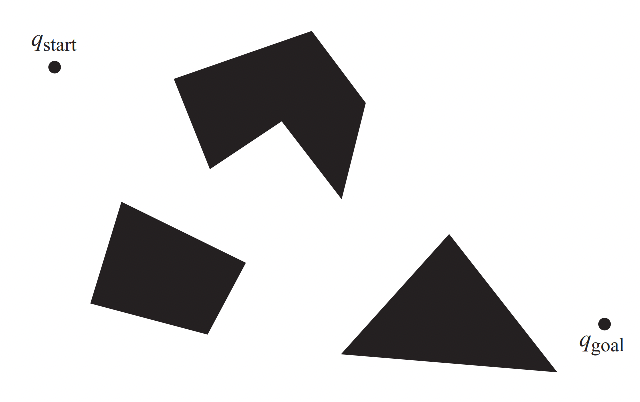
\includegraphics[width=60mm]{fig/fig_02_poly_cofig_space.png}
          \caption{A polygonal config space with start and goal}
          \label{fig:fig02}
        \end{figure}
       \end{center}
      \end{column}
    \end{columns}
    
  \end{frame}

  \begin{frame}{Visibility Graph}

    \begin{columns}
      \begin{column}[]{0.4\textwidth}
        The graph edges $e_{ij}$ are straight-line segments that connect two line-of-sight nodes $v_{i}$ and $v_{j}$
      \end{column}
      \begin{column}[]{0.6\textwidth}
        \begin{center}
        \begin{figure}
          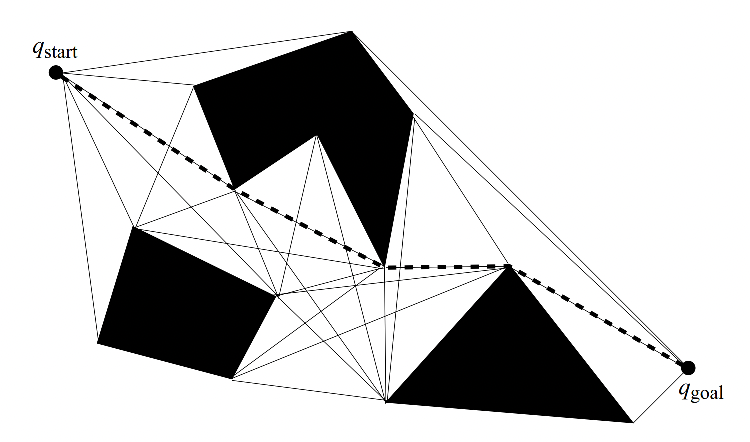
\includegraphics[width=60mm]{fig/fig_03_visibility_graph.png}
          \caption{The Visibility graph}
          \label{fig:fig03}
        \end{figure}
       \end{center}
      \end{column}
    \end{columns}
    
  \end{frame}

  \begin{frame}{Reduced Visibility Graph}

  the visibility graph has many needless edges. The use of supporting and separating lines can reduce the number of edges.

    \begin{columns}
      \begin{column}[]{0.4\textwidth}
        \begin{center}
          \begin{figure}
            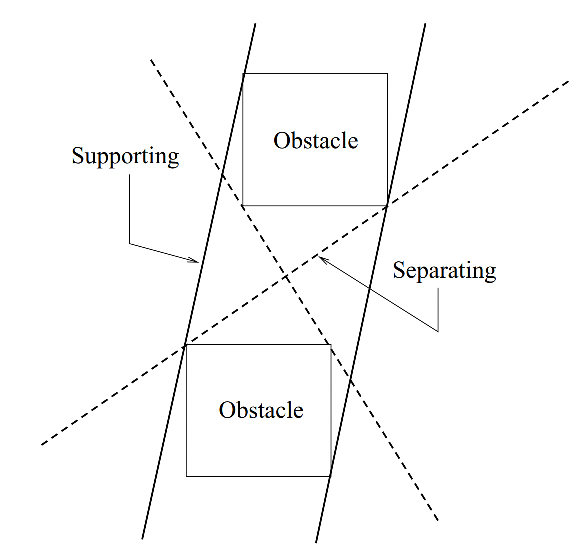
\includegraphics[width=40mm]{fig/fig_04_supporting_separating_segments.png}
            \caption{Supporting and Separating Line Segments}
            \label{fig:fig04}
          \end{figure}
         \end{center}
      \end{column}
      \begin{column}[]{0.6\textwidth}
        \begin{center}
        \begin{figure}
          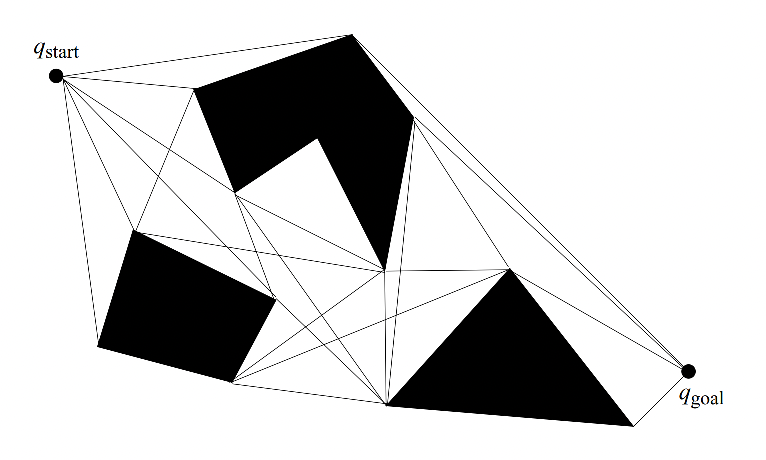
\includegraphics[width=60mm]{fig/fig_05_reduced_visibility_graph.png}
          \caption{Reduced Visibility graph}
          \label{fig:fig05}
        \end{figure}
       \end{center}
      \end{column}
    \end{columns}
    
  \end{frame}

  \begin{frame}
    \frametitle{Rotational Plane Sweep Algorithm}
  
    
  
  \end{frame}

  \subsection[Voronoi Diagrams]{Generalized Voronoi Diagrams}

  \begin{frame}
    \frametitle{Generalized Voronoi Diagrams}
    The \textbf{Generalized Voronoi Diagram} (\textbf{GVD}) is the set of points where the distance to the two closest obstacles is the same.
    \begin{center}
      \begin{figure}
        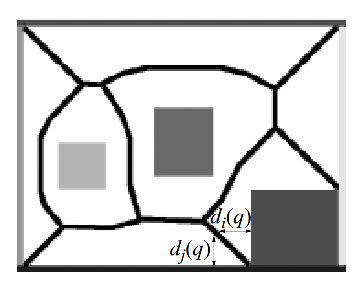
\includegraphics[width=60mm]{fig/fig_06_gvd.png}
        \caption{Voronoi Diagram}
        \label{fig:fig06}
      \end{figure}
     \end{center}
  
  \end{frame}

  \begin{frame}
    \frametitle{Construction of the GVD}
    \begin{center}
      \begin{figure}
        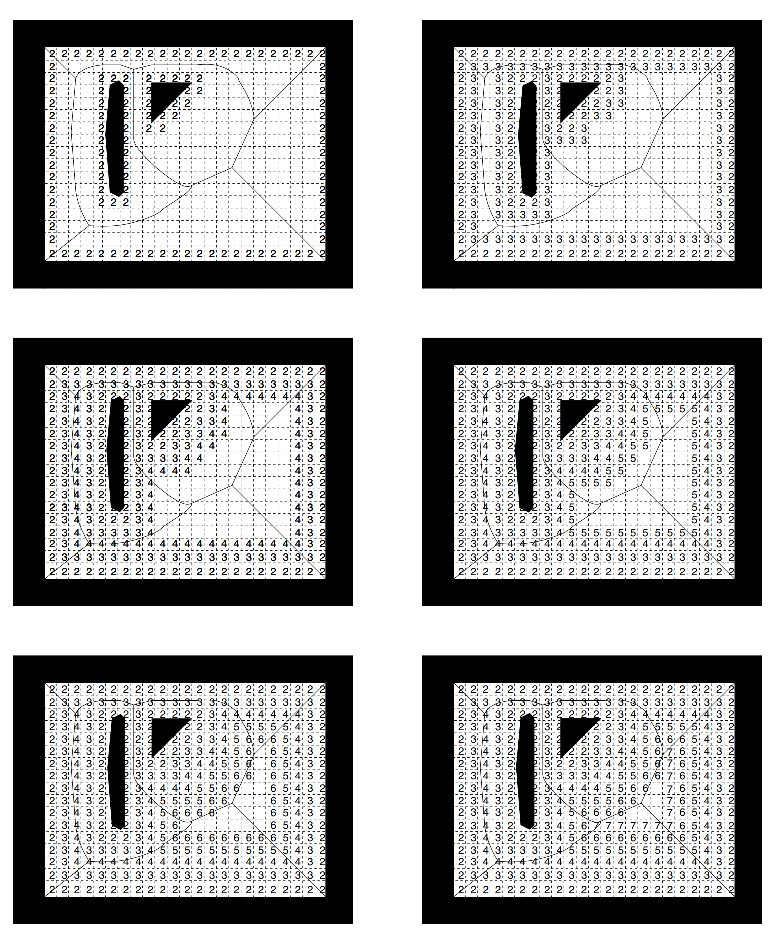
\includegraphics[width=55mm]{fig/fig_07_brushfire.png}
        \caption{The \textbf{Brushfire algorithm} uses a grid to approximate distance}
        \label{fig:fig07}
      \end{figure}
     \end{center}
  
  \end{frame}

  \section[Cell Decompositions]{Cell Decomposition}

  \section[Potential Field]{Potential Field}

\end{document}